%%if
\section{Exemple d'équation}
L'une des principales forces de \LaTeX~est la saisie d'équations. L'équation \ref{eq:1}, citée à titre d'exemple, représente la transformation de phase d'une lentille biconvexe. Pour rédiger une équation \LaTeX~vous pouvez utiliser des outils en ligne tels que \href{https://www.latex4technics.com/}{latex4technics}. Essayez autant que possible d'écrire vos équations à la main. La courbe d'apprentissage n'est pas très raide et la valeur ajoutée est grande. Vous pouvez vous aider du panneau de \LaTeX~Workshop dans Visual Studio Code. Il est accessible via le raccourcis clavier \keystroke{Ctrl} + \keystroke{Alt} + \keystroke{X}.

\begin{equation} \label{eq:1}
    \begin{split}
        L(x,y) &= \exp\left( - i\frac{{2\pi }}{\lambda }\left( {n\Delta \varphi (x,y) + \Delta {\varphi _0} - \Delta \varphi (x,y)} \right)\right)\\
        &= {\exp\left({i\frac{{2\pi }}{\lambda }\Delta {\varphi _0}}\right)}{\exp\left({ - i\frac{{2\pi }}{{\lambda f}}({x^2} + {y^2})}\right)}
    \end{split}
\end{equation}

\section{Exemples de diagrammes}

Les diagrammes de flux peuvent être réalisés en utilisant l'outil \href{https://app.diagrams.net/}{draw.io}. Une exportation en \texttt{.drawio} (non compressé) permet de garder les sources de la figure. Le rendu en \texttt{.pdf} sera réalisé à la volée à la compilation. L'intérêt est double : n'avoir qu'une source de vérité \cad pas d'image intermédiaire à stocker, et réduire la quantité d'information stockée.

Puisque la source est au format XML, les textes sont accessibles au correcteur orthographique et il vous est rendu possible les modifier sans avoir à éditer l'image. La figure \ref{euclide.drawio} en est un exemple.

\fig[H, width=9cm]{Algorithme d'Euclide}{euclide.drawio}

Notons qu'il est inutile d'insérer des images coloriées là où la couleur n'offre aucune valeur ajoutée ; évitez également les ombrages et autres effets de style. Enfin, préférez toujours des représentations vectorielles là où c'est possible.

Voici un autre type de diagramme utile (figure \ref{sequence.drawio}), celui d'une séquence UML.

\fig[H, width=0.4\textwidth]{Diagramme de séquence}{sequence.drawio}

Ce modèle apporte la commande \verb!\fig! qui peut prendre plusieurs options. Utilisez \verb!H! pour forcer la figure à apparaître à l'endroit de la déclaration. Ajustez la largeur de la figure à \SI{80}{\percent} de largeur de page avec \verb!width=0.8\textwidth!.

\section{Exemple de figure}

Pour présenter vos résultats d'expérience, vous pouvez soit dessiner des graphiques manuellement en utilisant des outils de dessin vectoriel comme Inkscape ou Adobe Illustrator, comme illustré à la figure \ref{plot.svg}.

\fig[H, width=0.8\textwidth]{Exemple de graphique plan}{plot.svg}

% Vous pouvez utiliser Python ou Matlab pour générer des figures à la volée à partir d'une source de données. À titre d'exemple, le code source \ref{python} permet de générer la figure \ref{bode.py}.
% \begin{listing}[h]
%     \inputminted{python}{assets/figures/bode.py}
%     \caption{Génération d'un diagramme de Bode \label{python}}
% \end{listing}

% \fig[H, width=12cm]{Diagramme de Bode généré à la volée}{bode.py}

\subsection{Example de schéma électronique}
Vous pouvez également utiliser TikZ pour créer vos propres schémas électriques et électroniques comme l'exemple \ref{circuit}. N'hésitez pas à vous inspirer d'exemples disponibles sur internet (\href{https://texample.net/tikz/examples/area/electrical-engineering/}{texample/electrical-engineering}).

\begin{figure}[h]
    \begin{center}
        \begin{circuitikz}
            \draw
            (0,0) to [short, *-] (6,0)
            to [V, l_=$\mathrm{j}{\omega}_m \underline{\phi}^s_R$] (6,2)
            to [R, l_=$R_R$] (6,4)
            to [short, i_=$\underline{i}^s_R$] (5,4)
            (0,0) to [open, v^>=$\underline{u}^s_s$] (0,4)
            to [short, *- ,i=$\underline{i}^s_s$] (1,4)
            to [R, l=$R_s$] (3,4)
            to [L, l=$L_{\sigma}$] (5,4)
            to [short, i_=$\underline{i}^s_M$] (5,3)
            to [L, l_=$L_M$] (5,0);
        \end{circuitikz}
        \caption{Circuit électrique \label{circuit}}
    \end{center}
\end{figure}

\subsection{Dessins techniques}
La présentation de dessins mécaniques est préférée en vue filaire. SolidWorks conserve la représentation vectorielle à l'exportation mais pas lorsqu'il y a des textures ou des rendus. À partir du PDF généré, l'image peut être isolée et sauvegardée en format SVG.

\begin{figure}[!ht]
    \begin{center}
        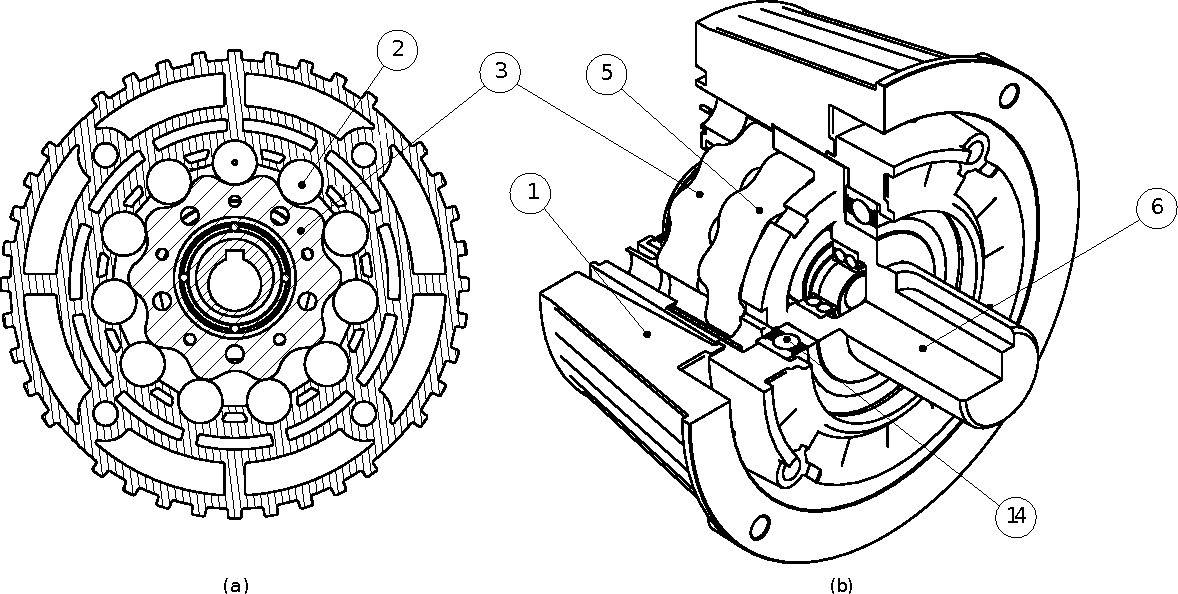
\includegraphics[width=10cm]{\assetsdir/assembly.svg.pdf}
    \end{center}
    \caption[Assemblage mécanique]{\label{assembly}Réducteur cycloïdale de puissance comportant 6. l'axe de sortie, 14. le roulement de sortie, 1. le corps du réducteur en aluminium, 3 et 5. les disques cycloïdaux et 2. les goupilles de prise... D'autres informations liées à la figure elle-même peuvent aussi figurer dans la légende}
\end{figure}

Notez ici que la légende est particulièrement longue. Celle que vous retrouverez dans la table figures est plus courte. La commande \mintinline{latex}{\caption[courte]{longue}} permet de saisir une légende courte pour la table des figures et une légende longue pour documenter la figure. Utilisez \mintinline{latex}{\fig[short=Légende courte]{Légende longue}{fichier}}.

La figure \ref{assembly} est un dessin technique épuré qui permet de décrire un phénomène ou un fonctionnement important dans le rapport technique. Les mises en plan détaillées seront quant à elles disponibles en annexes.

\section{Tableaux}

Concernant les tableaux un seul conseil : restez simple et minimaliste, n'ajoutez des séparateurs que là ou c'est nécessaire pour améliorer la lisibilité. Une liste de quelques cantons suisses est donnée à titre d'exemple dans la table \ref{cantons}.

\begin{table}[h]
    \begin{center}
        \caption{Liste des cantons \label{cantons}}
        \begin{tabular}{c|l|r}
            Abréviation & Nom du canton & Depuis                  \\ \hline
            ZH          & Zürich        & \ordinalnum{1} mai 1351 \\
            BE          & Berne         & 6 mars 1353             \\
            FR          & Fribourg      & 22 décembre 1481        \\
            VD          & Vaud          & 19 février 1815         \\
            VS          & Valais        & 4 août 1815             \\
            NE          & Neuchâtel     & 19 mai 1815             \\
            GE          & Genève        & 19 mai 1815
        \end{tabular}
    \end{center}
\end{table}

Comparez la lisibilté de cette même table avec celle que vous pourriez trouver dans un document Word :

\begin{table}[h]
    \begin{center}
        \caption{Liste des cantons (vilain)}
        \begin{tabular}{|l|l|l|} \hline
            \textbf{Abréviation} & \textbf{Nom du canton} & \textbf{Depuis}         \\
            \Xhline{4\arrayrulewidth}
            ZH                   & Zürich                 & \ordinalnum{1} mai 1351 \\ \hline
            BE                   & Berne                  & 6 mars 1353             \\ \hline
            FR                   & Fribourg               & 22 décembre 1481        \\ \hline
            VD                   & Vaud                   & 19 février 1815         \\ \hline
            VS                   & Valais                 & 4 août 1815             \\ \hline
            NE                   & Neuchâtel              & 19 mai 1815             \\ \hline
            GE                   & Genève                 & 19 mai 1815             \\ \hline
        \end{tabular}
    \end{center}
\end{table}

Si vous devez donner une spécification technique, n'oubliez pas de mentionner les valeurs minimales, maximales et nominales sans omettre l'unité de mesure. Notez que les séparateurs verticaux sont souvent critiqués pour réduire la lisibilité mais parfois ils sont utiles. Utilisez-les avec parcimonie. Jouez avec l'alignment des colonnes pour accroître la lisibilité et utilisez l'environmement \mintinline{latex}{tabularx} pour plus d'unité dans les largeurs de vos tableaux.

\begin{table}[h]
    \begin{center}
        \caption{Exigences techniques \label{specification}}
        \begin{tabularx}{\textwidth}{cXcccr}
            \toprule
            No. & Exigence                                                                   & Min. & Nom. & Max. & Unité                           \\
            \midrule
            E1  & Tension d'alimentation                                                     & 12   & 24   & 48   & \si{\volt}                      \\
            E2  & Fréquence                                                                  & 50   &      & 60   & \si{\hertz}                     \\
            E3  & Concentration                                                              &      & 300  & 1200 & \si{\nano\gram\per\milli\litre} \\
            E4  & \multicolumn{5}{l}{Doit pouvoir être stoppé à l'aide d'un arrêt d'urgence}                                                        \\
            \bottomrule
        \end{tabularx}
    \end{center}
\end{table}

L'exemple de la table \ref{specification}, assigne pour chaque exigence un numéro unique. Cette table est \textbf{normative}, chaque élément doit pouvoir être référencé par un identifiant unique (cf. T\ref{specification}-E3). Dans le cas ou cet identifiant est utilisé en dehors de ce document, la version du document devra être renseignée.

\section{Index}
\LaTeX~ permet d'indexer les mots \index{mots} importants. Il suffit de placer les termes importants d'un paragraphe dans la commande \mintinline{latex}{\index{terme}} et ils apparaîtront automatiquement à la fin de ce rapport dans l'index du document.

\index{Napoléon}

Imaginons que dans cette section nous parlions du cheval blanc \index{cheval blanc} de Napoléon. Il se pourrait que le lecteur recherche ce passage dans la version imprimée du rapport. Avec l'index, rien de plus facile. Allez jeter un oeil à la page \pageref{index}.

\section{Notes de bas de page}

\maraja{Je suis une marginale, et je suis utile pour résumé un paragraphe en quelques mots.} Parfois, il est plus élégant d'annoter une définition en utilisant une note de bas de page \footnote{La note en bas de page (ou note de bas de page) est une forme littéraire, consistant en une ou plusieurs lignes ne figurant pas dans le texte.}. Alternativement il est possible d'annoter un paragraphe avec une note marginale.

\section{Glossaire et acronymes}

La \Gls{heig-vd} membre de la \Gls{hes-so} propose ce modèle de document. Le format \LaTeX~est particulièrement adapté pour les documents qui contiennent des expressions mathématiques. Pour plus de détail sur l'utilisation d'un glossaire, se référer à \href{https://www.overleaf.com/learn/latex/Glossaries}{Overleaf/Glossaires}. Tient donc, ci-dessus nous utilisons deux acronymes. Les trouverez-vous dans le glossaire en page \pageref{glossaire} ?

\section{Unités de mesure}

Lorsque vous mentionnez des quantités, utilisez les unités du système international. \LaTeX~et le paquet \texttt{siunitx} permet la saisie de quantités. La commande suivante permet d'afficher \SI{42.12}{\kilo\gram\metre\per\square\second}.\par

\mintinline{latex}{\SI{42.12}{\kilo\gram\metre\per\square\second}}\par

Notez qu'une espace fine précède l'unité et que ces dernières ne sont pas en italiques.
%%fi